\begin{center}
\begin{tikzpicture}
    \node[anchor=south west,inner sep=0] (image)  at (0,0) {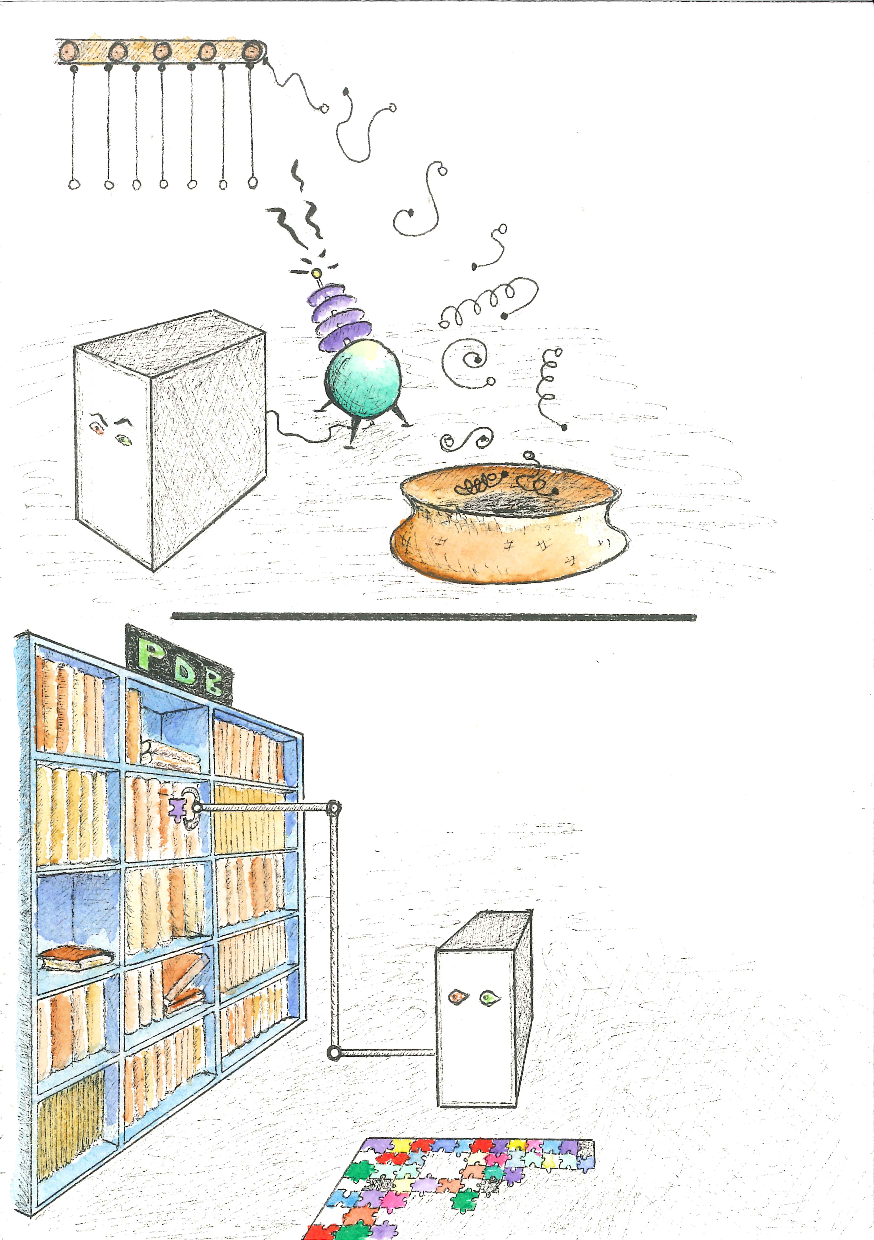
\includegraphics[trim={2mm, 2mm, 2mm, 2mm}, width=0.995\pagewidth]{scans/pan-4.pdf}};
    
   
    \begin{scope}[x={(image.south east)},y={(image.north west)}]
        \if\helplines1
        	\draw[help lines,xstep=.1,ystep=.1] (0,0) grid (1,1);
        \fi

        \node[align=justify, anchor=north west, text width=0.4\pagewidth](en) at (0.54, 0.95) {\english{One option is \emph{ab-initio}: starting from scratch, try a lot of different configurations, until one seems to match.}};
        
        \node[align=justify, anchor=north west, text width=0.55\pagewidth](en) at (0.38, 0.45) {\english{The other option is \emph{homology}, where the computer uses pieces from other proteins similar in sequence, for which we have the structure. Like pieces of a puzzle.}};
        
        % % %
        
        \node[align=justify, anchor=north west, text width=0.30\pagewidth](es) at (0.65, 0.8) {\spanish{Una opción es \emph{ab-initio}: empezando de cero, probando muchas configuraciones diferentes, hasta que alguna parezca coincidir.}};
        
    
        \node[align=justify, anchor=north west, text width=0.27\pagewidth](es) at (0.65, 0.35) {\spanish{La otra opción es \emph{por homología}: donde el ordenador busca en la base de datos de estructuras de proteínas por algunas similares a la nuestra, y los usa como piezas de puzle.}};
    \end{scope}

\end{tikzpicture}
\end{center}